\documentclass[12pt]{article}
\usepackage{latexblog}

% ============================================================
% Blog Metadata
% ============================================================
\blogtitle{调试JDK源码}
\blogdate{2020-01-25}
\blogtags{刨根问底, 探索分析, JDK1.8, Series-JDK-Source}
\bloglang{zh}
\blogsummary{}

\begin{document}
\makeblogtitle

最近想要直接调试下JDK的源码却发现有些变量不能显示，像这样：

\begin{figure}
\centering
\pandocbounded{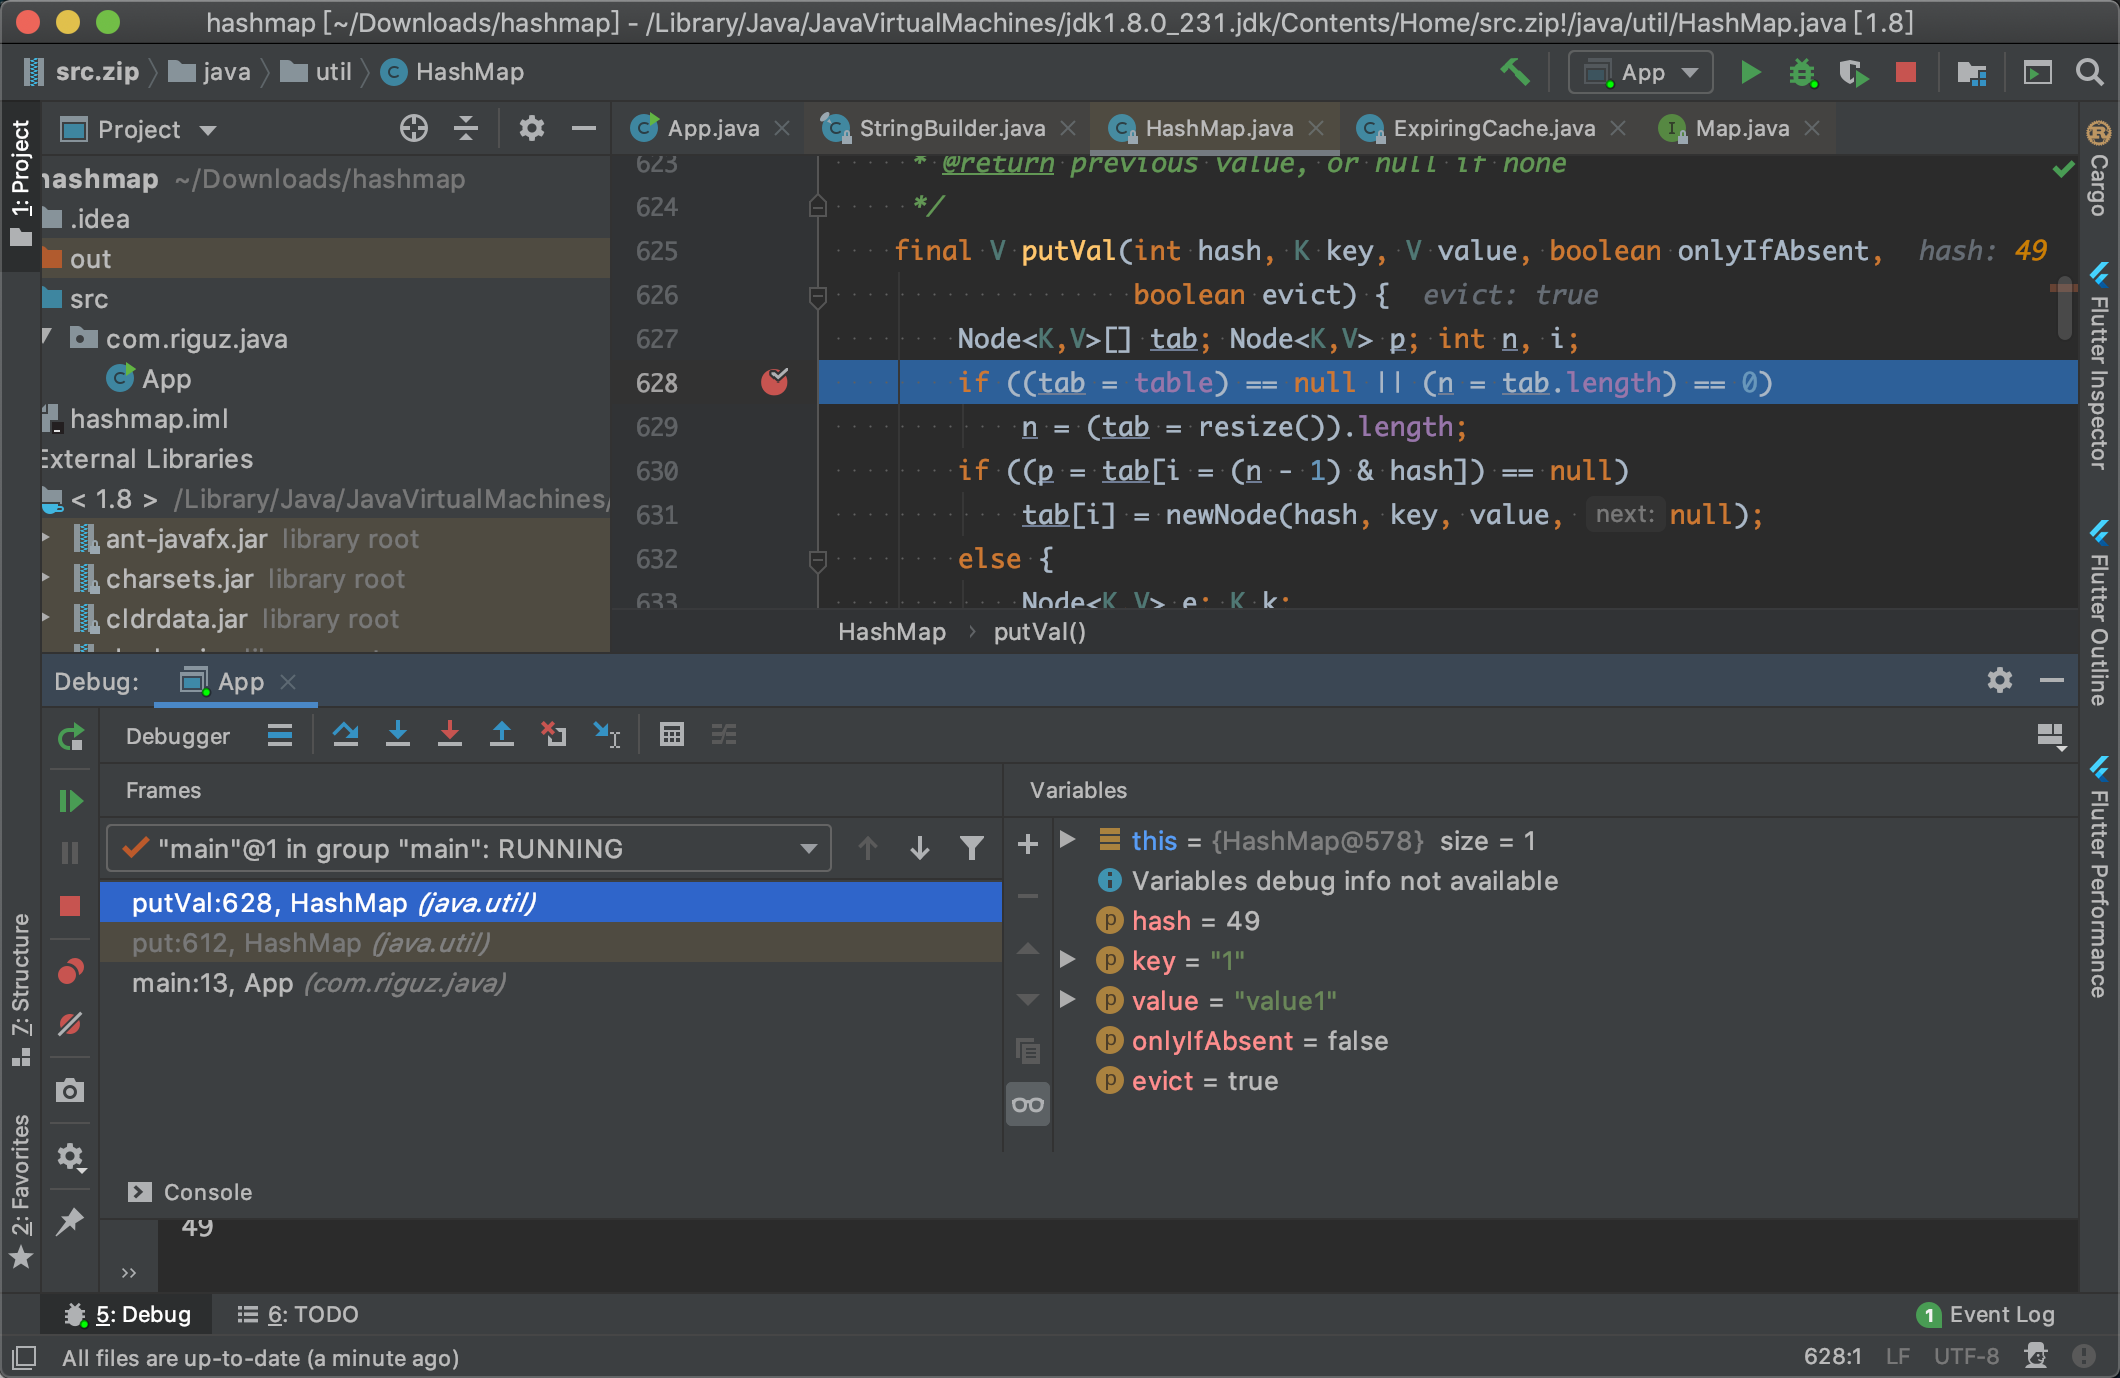
\includegraphics[keepaspectratio,alt={IntelliJ}]{images/Intellij-no-debuginfo.png}}
\caption{IntelliJ}
\end{figure}

其原因是因为JDK中的rt.jar在release的时候没有附带调试信息。所以解决这个问题的思路是这样的：

\begin{itemize}
\tightlist
\item
  重新编译你想要调试的类(\texttt{javac\ -g})
\item
  将带调试信息的类覆盖原来的
\item
  重新进行调试
\end{itemize}

实际上，在IntelliJ中操作起来可能比较简单，可以分为以下几步：

\begin{itemize}
\tightlist
\item
  将jdk的源码从JDK中拷贝出来，例如/Library/Java/JavaVirtualMachines/jdk1.8.0\_231.jdk/Contents/Home/src.zip
\item
  将源码解压，并将其中\texttt{java},\texttt{javax}两个文件夹拷贝到一个空的Java工程中
\item
  编译源码，IntelliJ默认设置编译是包含了调试信息的。编译完成之后，将其\href{https://www.jetbrains.com/help/idea/packaging-a-module-into-a-jar-file.html\#}{导出到jar包}中。
\item
  将导出的jar包（比如说rt\_debug.jar)放入到\texttt{\$JAVA\_HOME/jre/lib/endorsed}文件夹下面即可。如果这个目录不存在，手动创建一下。
\item
  重新进行调试即可。
\end{itemize}

\begin{figure}
\centering
\pandocbounded{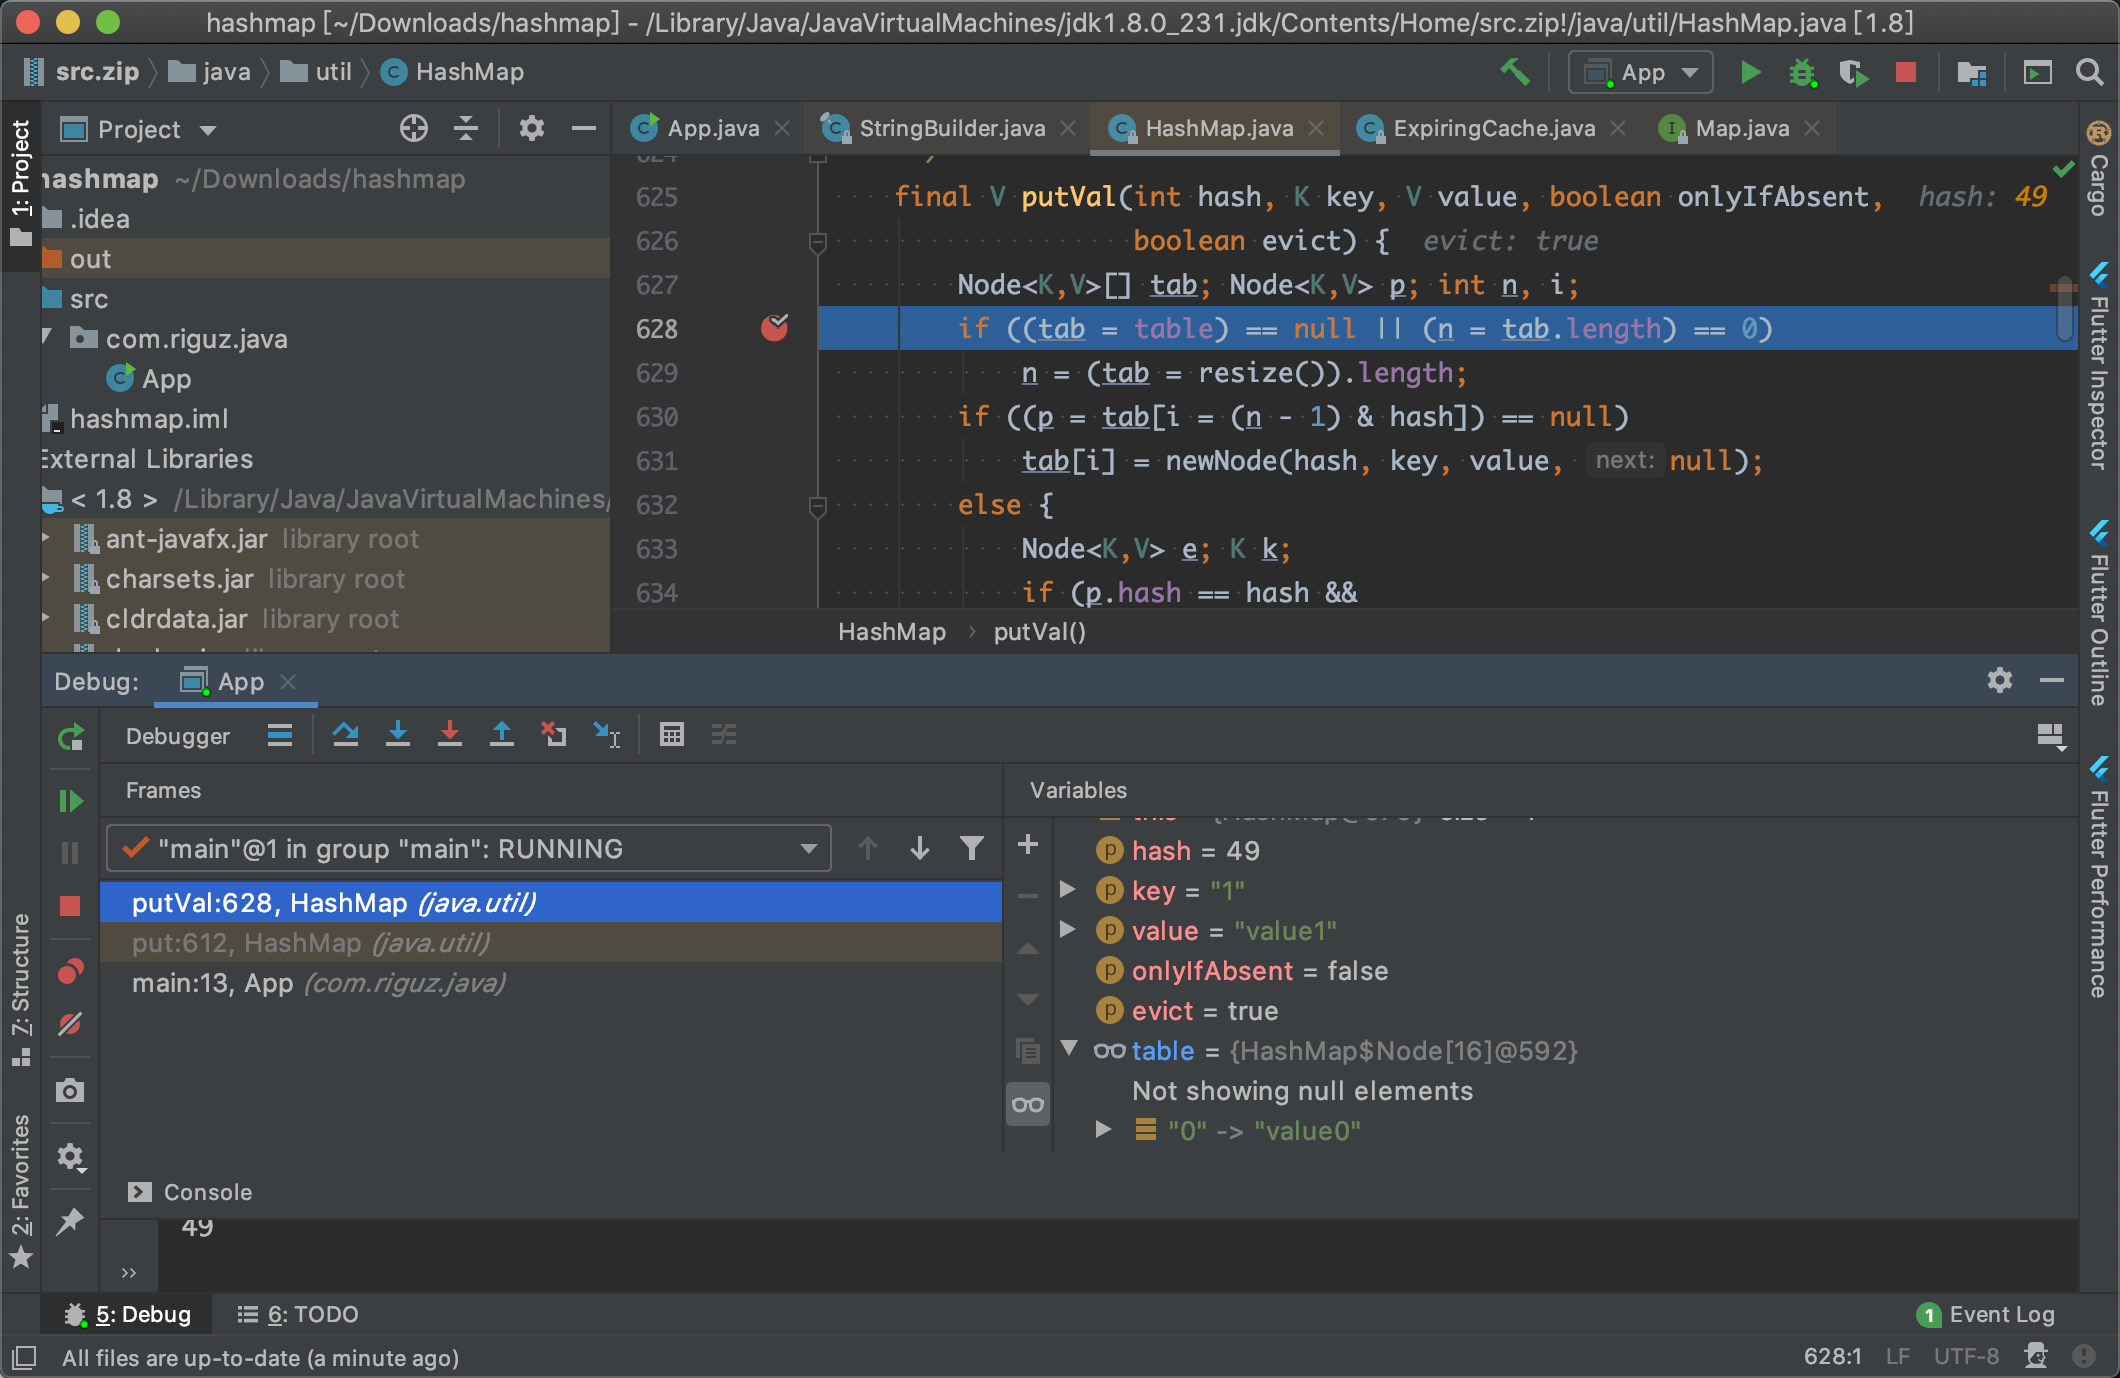
\includegraphics[keepaspectratio,alt={IntelliJ}]{images/Intellij-with-debuginfo.png}}
\caption{IntelliJ}
\end{figure}

事实上，这里利用了\texttt{endorsed-standards\ override\ mechanism}这一个JVM特性来重载了Java的类，这个特性已经在Java8中被deprecated了(\href{https://www.java.com/en/download/faq/release_changes.xml}{release notes for Java 8 Update 40 (8u40)})，但是Java8中仍然可用。

\begin{quote}
The endorsed-standards override mechanism and the extension mechanism are deprecated and may be removed in a future release. There are no runtime changes. Existing applications using the `endorsed-standards override' or `extension' mechanisms are recommended to migrate away from using these mechanisms.
\end{quote}

Reference:

\begin{itemize}
\tightlist
\item
  \href{https://stackoverflow.com/questions/1313922/step-through-jdk-source-code-in-intellij-idea}{Step through JDK source code in IntelliJ IDEA}
\item
  \href{https://stackoverflow.com/questions/18255474/debug-jdk-source-cant-watch-variable-what-it-is}{debug jdk source can't watch variable what it is}
\end{itemize}


\end{document}
